\setlength{\footskip}{8mm}

\chapter{Results}

\label{ch:results}

This chapter describes the results obtained with this research.
First, the deep neural network model used in the study is described. Then, the results obtained with this network in the context of face verification are given. Finally, we will describe the final experimental software which is available online and the results one can expect with it.

\section{Preliminary results}
Before the proposal, some parts of the solution have been built.
\begin{itemize}
\item Scripts to generate the database of face images from a video surveillance sequence have been written. The database has been generated and is usable for a direct face identification model. However, the overlap calculation for face detection is not written yet. Hence, the number of available classes is limited, decreasing the performances of a \enquote{Same/Not Same} network. The direct face identification model is not be affected by this issue, however it can be built with the current version of the database. The database contains 55,203 images. After manual labeling of the faces in the database, 183 images were labeled 1 for the first researcher, 325 were labeled 2, 15 were labeled 3.
\item The scripts to generate the database files mentioned in Figure 3.2 are fully written, and work both for a direct face identification and for a Siamese network. They were executed for this second scenario. Four files \enquote{train1.txt}, \enquote{train2.txt}, \enquote{test1.txt}, and \enquote{test2.txt}, as described in section 3.6.2, were built.
\item A Siamese model has been designed with Caffe and was trained on the generated database for 50,000 epochs. This training took a night, with batches of size 20, on the 780 GTX GPU card given by the laboratory. The accuracy of the resulting network could not be tested yet because of the singular output generated by such a network, as mentioned in section 2.3.1. A script is being written to face this issue.
\end{itemize}

\section{Network used in this research}

Wu, He and Sun published a light convolutional neural network for face verification (November 2015). Its particularity is that it is extremely light but still reaches state-of-the-art results.

\subsection{Architecture}
The following figure describes its architecture.

\begin{figure}[!ht]
  \centering
  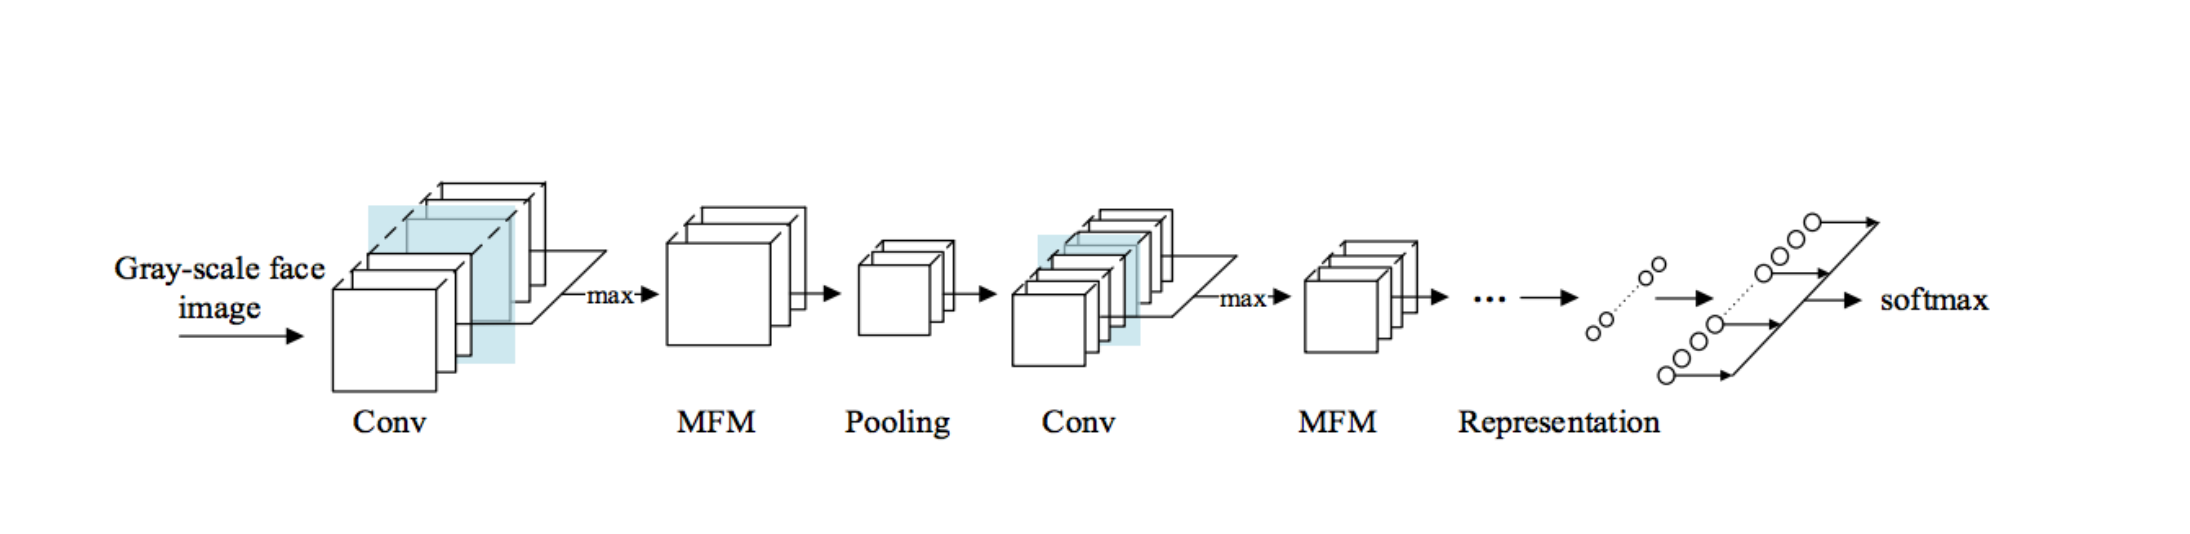
\includegraphics[scale=0.4]{figures/final_net.png}  
  \caption[Architecture of the lightened convolution network. Extracted from Wu, He, Sun, 2015.]{Architecture of the lightened convolution network. Extracted from Wu, He, Sun, 2015.}
  \protect\label{fig:Siamese}
\end{figure}
\FloatBarrier
\end{itemize}

First, as an input, a Gray-scale face image is provided. The article suggests the use of two possible models. The one used in this research is built with 4 convolution layer with Max-Feature-Map activation functions, 4 max-pooling layers and 2 fully connected layers. The details are given in the following figure.

\begin{figure}[!ht]
  \centering
  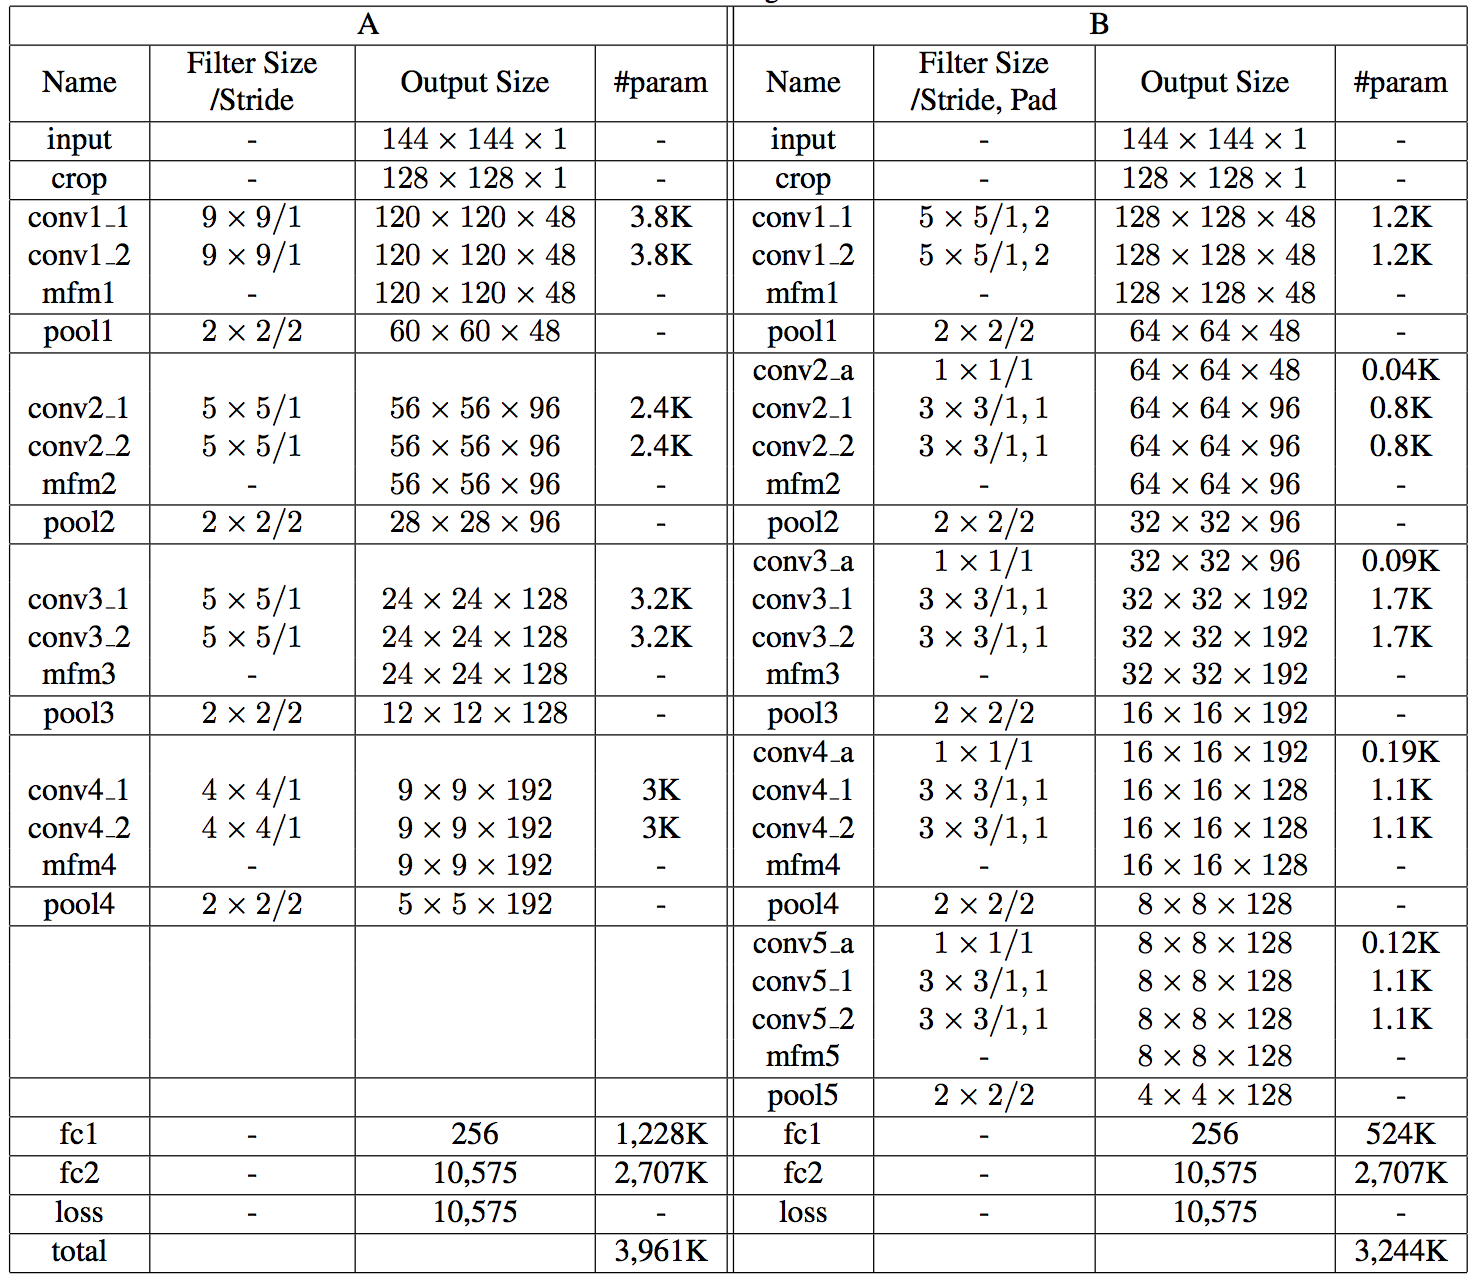
\includegraphics[scale=0.6]{figures/architecture.png}  
  \protect\label{fig:architecture}
  \caption[Details on the architecture of the lightened convolution networks. Extracted from Wu, He, Sun, 2015.]{Details on the architecture of the lightened convolution networks. Extracted from Wu, He, Sun, 2015.}
\end{figure}
\FloatBarrier
\end{itemize}

\FloatBarrier

The MFM function works as explained in the following figure.

\begin{figure}[!ht]
  \centering
  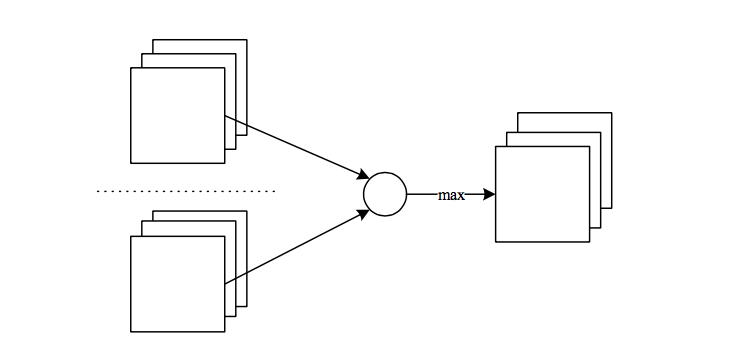
\includegraphics[scale=0.4]{figures/mfm.png}  
  \protect\label{fig:mfm}
  \caption[The MFM activation function used on a convolution layer. Extracted from Wu, He, Sun, 2015.]{The MFM activation function on a convolution layer. Extracted from Wu, He, Sun, 2015.}
\end{figure}
\FloatBarrier
\end{itemize}

\FloatBarrier

Given a convolution layer \(C \in R^h^w^2^n\), the MFM can be written :

\begin{figure}[!ht]
  \centering
  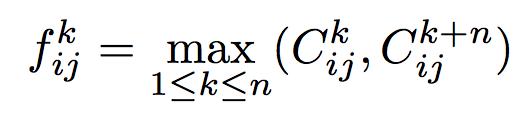
\includegraphics[scale=0.4]{figures/equ.png}  
  \protect\label{fig:equ}
\end{figure}
\FloatBarrier
\end{itemize}

\FloatBarrier

\(2n\) being the channel of the input convolution layer, \(1 \leq i \leq h\) and \(1 \leq j \leq w\).


\subsection{Results}

As said previously, these networks reach state-of-the-art results. The two networks were trained on the LFW database and tested both on LFW and YTF (YouTube Faces Database). The results are given in the next two tables, compared with other state-of-the-art methods.

\begin{figure}[!ht]
  \centering
  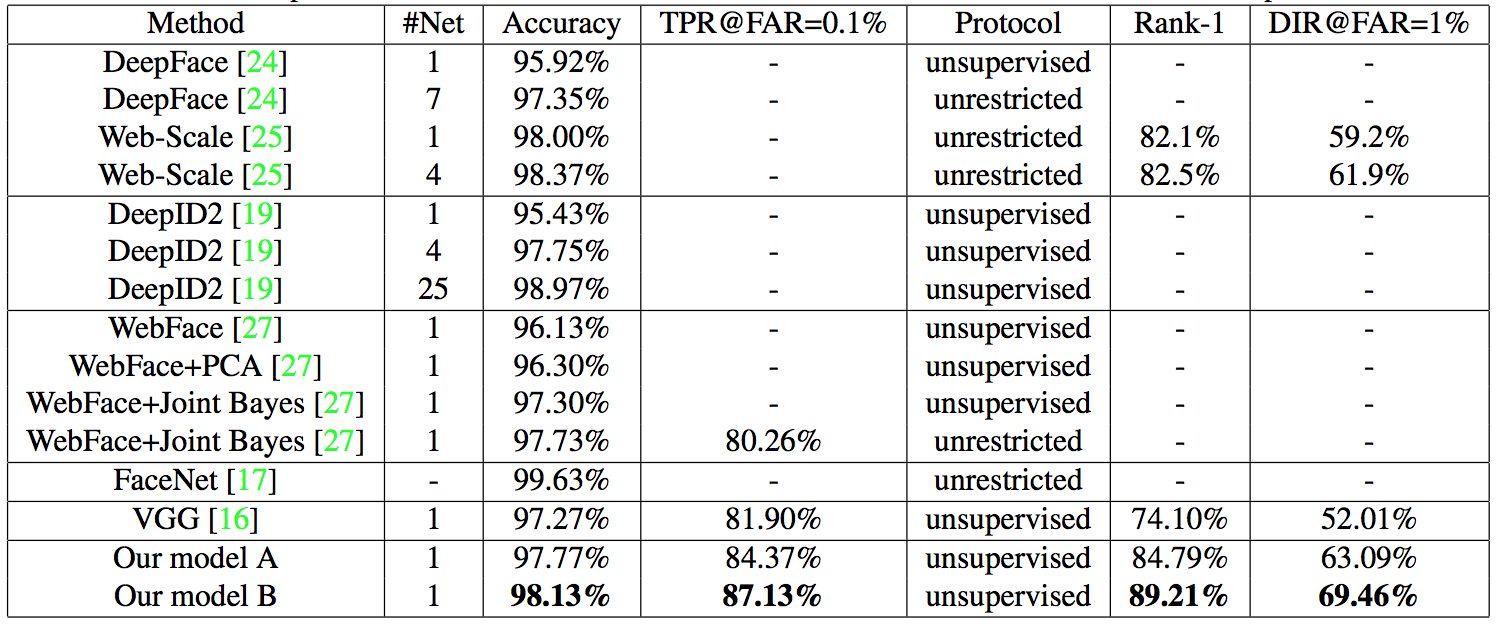
\includegraphics[scale=0.6]{figures/lfw.png}  
  \protect\label{fig:mfm}
  \caption[Comparison with other state-of-the-art methods on LFW. Extracted from Wu, He, Sun, 2015.]{Comparison with other state-of-the-art methods on LFW. Extracted from Wu, He, Sun, 2015.}
\end{figure}
\FloatBarrier
\end{itemize}


\begin{figure}[!ht]
  \centering
  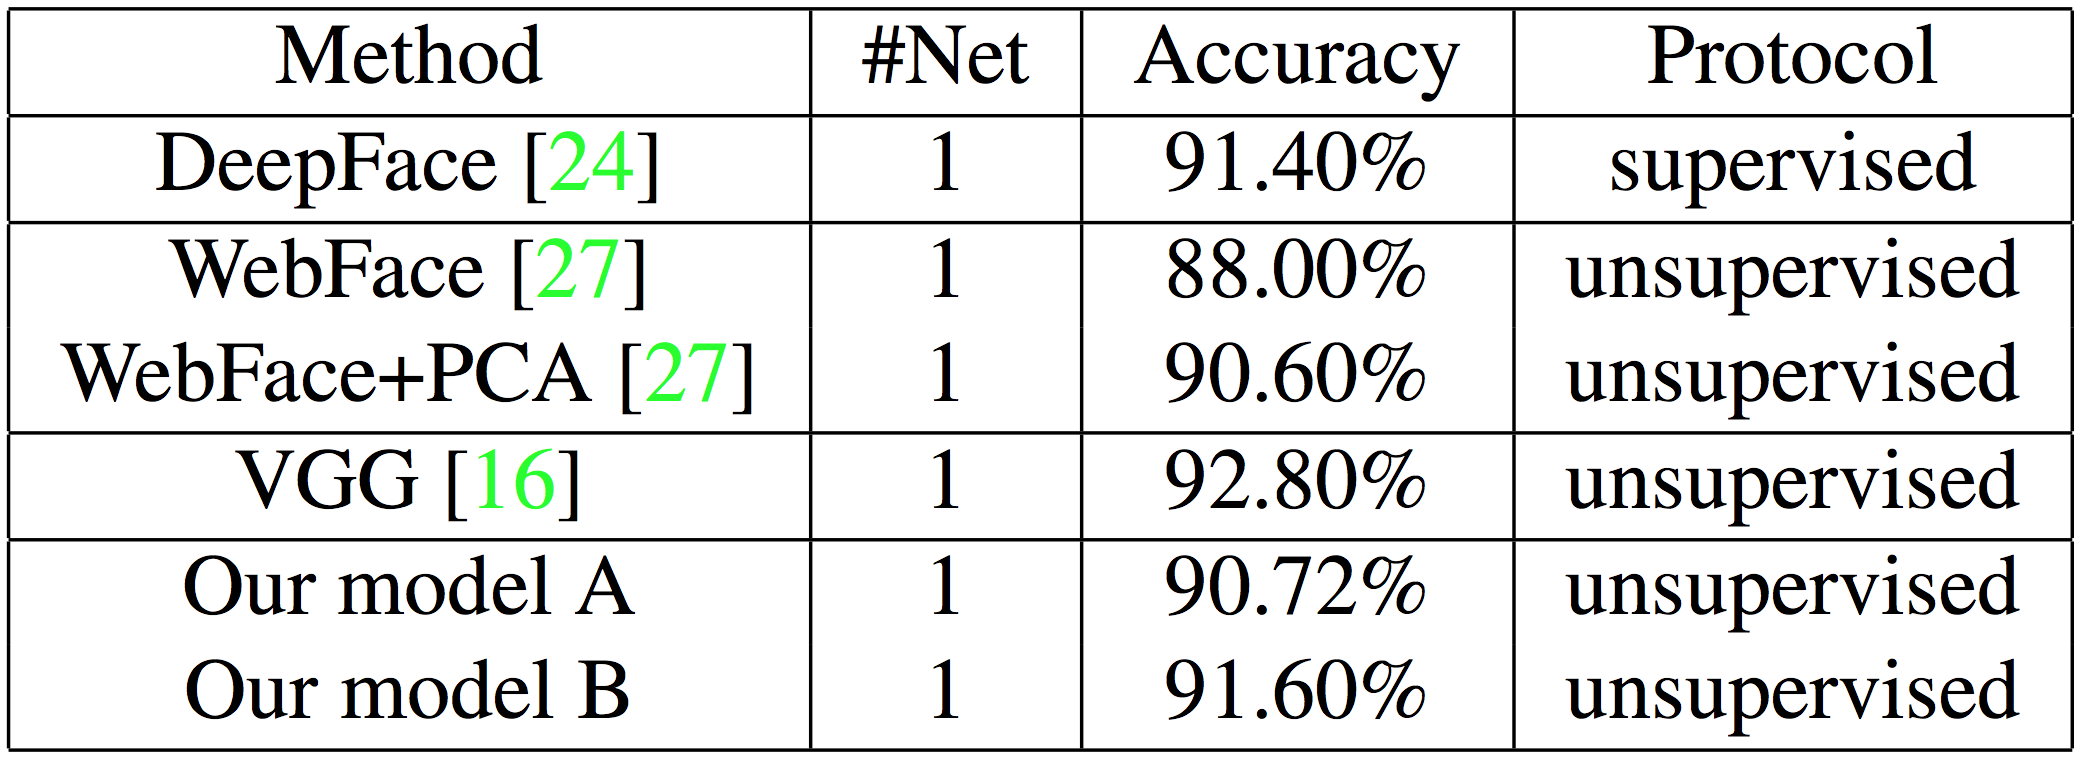
\includegraphics[scale=0.3]{figures/ytf.png}  
  \protect\label{fig:mfm}
  \caption[Comparison with other state-of-the-art methods on YTF. Extracted from Wu, He, Sun, 2015.]{Comparison with other state-of-the-art methods on YTF. Extracted from Wu, He, Sun, 2015.}
\end{figure}
\FloatBarrier
\end{itemize}

\FloatBarrier

